% Copyright (C) 2012,2013 The ESPResSo project
%  
% This file is part of ESPResSo.
%   
% ESPResSo is free software: you can redistribute it and/or modify it
% under the terms of the GNU General Public License as published by the
% Free Software Foundation, either version 3 of the License, or (at your
% option) any later version.
%  
% ESPResSo is distributed in the hope that it will be useful, but
% WITHOUT ANY WARRANTY; without even the implied warranty of
% MERCHANTABILITY or FITNESS FOR A PARTICULAR PURPOSE.  See the GNU
% General Public License for more details.
%  
% You should have received a copy of the GNU General Public License
% along with this program.  If not, see <http://www.gnu.org/licenses/>.
%
\documentclass[a4paper]{article}
\usepackage{graphicx}
\usepackage{verbatim}
%\usepackage{minipage}

\title{Implementation of object-in-fluid in ESPResSo}
\author{Ivan Cimr\'ak$^\star$, Markus Gusenbauer$^\dagger$\\
\ \\
$^\star$ Department of Software Technologies, University of \v Zilina, Slovakia\\
$^\dagger$ St. Poelten University of Applied Sciences, Austria}
\date{}
\begin{document}
\maketitle
\section{Object-in-fluid in 5 minutes}
The following lines are from the official webpage of ESPResSo:
\begin{center}
\begin{minipage}{0.9\textwidth}
\emph{
"ESPResSo is a highly versatile software package for performing and analyzing scientific Molecular Dynamics many-particle simulations of coarse-grained atomistic or bead-spring models as they are used in soft-matter research in physics, chemistry and molecular biology. It can be used to simulate systems such as polymers, liquid crystals, colloids, ferrofluids and biological systems, for example DNA and lipid membranes."}
\end{minipage}
\end{center}
These lines tell the user exactly, what ESPResSo is aimed for. Molecular simulations. Very briefly: given the points in the space, and given the forces between them (and how they depend on many parameters), ESPResSo can compute how these points move in space (and much more, of course).

Probably all current simulations using ESPResSo, work with objects (molecules, atoms, polymers, colloids, crystals, ...) that are physicaly composed of points linked together with bonds. These objects are like skeletons, without inner or outer volume. 

Our idea is to use ESPResSo for objects that do have inner volme, for example red blood cells, magnetic beads, capsules, ... In fact, it is easy: the boundary of an object (for example a red blood cell) is covered with triangular mesh. The vertices of the mesh are put into ESPResSo as particles. The edges of the mesh will define elastic forces keeping the shape of the red blood cell. The movement of the red blood cell will be achieved by adding forces to the mesh points and voil\'a, we have moving object simulated in ESPResSo.

\section{Objects in a fluid}
Modelling of the flow of a fluid with immersed elastic or rigid objects is a challenging task. The fluid interacts with an elastic object resulting in its deformation; this imediately generates forces acting back on the fluid. The aim is to describe the immersed object using the notion of particles, and to create bonds between these particles representing elastic or rigid forces. Such an object is put in a Lattice-Boltzman flow.

We consider objects composed of a membrane encapsulating the fluid inside the object. For now, the inside fluid must have the same density and viscosity as the outside fluid. (See Section \ref{subsec:viscosity} with unresolved issues.) The object will be represented by its membrane (boundary) and the membrane will be discretized using a triangulation. Such a triangulation will define particles distributed on the surface of the immersed object. Next we define different bonded interactions: 
\begin{itemize}
\item between two particles, corresponding to the edges in the triangulation (modelling the stretching of the membrane), 
\item between three particles, corresponding to the triangles of the triangulation (local area, or local surface preservation of the membrane), 
\item between four particles, corresponding to two triangles from the triangulation sharing a common edge (bending of the membrane). 
\end{itemize}

The object immersed  in the fluid will move under the influence of the deforming forces, defined through the bonds, and under the influence of the fluid motion. The fluid-particle interaction is described in the user guide of ESPResSo. We use the same approach. This interaction is based on the frictional force between the fluid and the spherical particles. In our case however, we consider the movement of a larger immersed object and the particles are only a virtual discretization points on the surface of the object. Therefore the object will move in the flow only if there is a nonzero difference between the fluid velocity and the particle velocity. In other words, there has to be at least small flow through the membrane, which is in most cases unphysical. However, we believe that on larger scales, this unphysical flow through the membrane is negligible.

Other approach (See Section \ref{subsec:coupling} with unresolved issues) is to use the no-slip condition on the boundary of the immersed object. In this case, the influence of the fluid on the immersed object is not transferred through the forces, but through the velocities of the particles on the membrane. This is completely different approach, however the flexibility of ESPResSo allows for implementing it. See unresolved issues.

\subsubsection*{Membranes}
With our approach it is easy to model also elastic sheets, or free membranes that do not necessarily enclose a 3D object. In this case, we do not define area\_{}force\_{}global and volume\_{}force interactions, since these two interactions are ment for closed immersed objects.

\subsubsection*{Parameters}
There are several parameters involved in this model. All of them should be calibrated. 
\begin{itemize}
\item Mass of the particles. Every particle has its mass and the dynamics is influenced by this parameter. 
\item Friction coefficient. The main parameter describing the fluid-particle interaction is the \verb friction \ parameter from the ESPResSo command \verb lbfluid .
\item Parameters of elastic moduli. Elastic behaviour can be described by different eleastic moduli. We show five of them: stretching, bending, local and global area preservation and volume preservation. Each of them has its own scaling parameter, we denote them $ks, kb, kal, kag, kv$, respectively.
\end{itemize}
The mass of the particles and the friction coefficient can be calibrated using the drag coefficients of the ellipsoidal objects. These drag coefficients have known analytical values and the mass and friction can be calibrated to fit this values. More details about the calibration is in \cite{Cimrak2011a}.

The elastic parameters are specific to the immersed onjects. They correspond to their physical values. More details about their mechanical and biological meaning is presented in \cite{Dao2003} specifically for red blood cells. However, the proper calibration to fit the experimental data has been performed in \cite{Cimrak2011a}.

\subsection{Geometry}
The membrane of the immersed object is triangulated. In Figure \ref{fig:rbc} you can see an example of such triangulation. 
\begin{figure}[t]
   \centering
      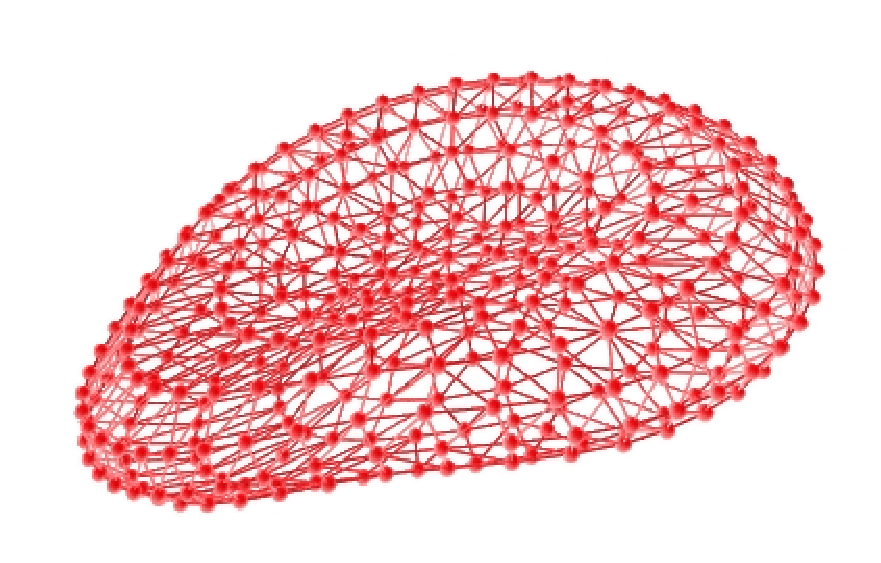
\includegraphics[width=0.45\textwidth]{figures/bloodCell.eps}
      \caption{Triangular mesh representing the boundary of a RBC deformed in the fluid flow.}
  \label{fig:rbc}
\end{figure}
Triangulation can be obtained using various software tools. Two files must be available for the tcl script: \verb nodes.dat \ and \verb triangles.dat . The parameters of the mesh, such as the number of particles on the surface of the immersed object are determined from the file \verb nodes.dat \  by counting its lines. Also, number of triangles in the mesh is determined by counting the number of lines in file \verb triangles.dat \ .

The \verb nodes.dat \ contains thus \verb nnode \ lines with three real numbers separated by blank space, representing three coordinates of the corresponding particle. The membrane is thus discretized into \verb nnode \ particles with IDs starting from 0 to \verb nnode-1 . The IDs are assigned in the same order as in the \verb nodes.dat \ file. 

The \verb triangles.dat \ contains \verb ntriangle \ lines with three nonnegative integers separated by blank space. Each line represents one triangle in the triangulation. For algorithmic purposes it is crucial to have defined a correct orientation of the triangle. We define the orientation using the normal vector associated with the triangle. The important rule is that the normal vector of the triangle must points inside the immersed object.

As an example, let us have one line in the file \verb mesh-triangles.dat \ with numbers 4, 0 and 7. This means that particles with IDs 4, 0 and 7 form one triangular face of the triangulation. The orientation is defined as follows: create two vectors $v_1$ and $v_2$, such that $v_1$ is pointing from particle 4 to particle 0, and $v_2$ is pointing from particle 4 to particle 7. Be carefull, the order of vectors and particles matters!

The normal vector $n$ is computed as a vector product $v_1 \times v_2$. The direction of $n$ can be determined by the rule of right hand: the thumb points in the $v_1$ direction, the index finger in the $v_2$ direction and the middle finger in the $n$ direction. Following this principle, all the lines in the \verb triangles.dat \ file must be such that the normal vectors of the corresponding triangles must point inside the immersed object.

These two files are sufficient to describe the geometry and topology of the triangulation. For the definition of bonded interactions the following geometric entities are necessary: position of the particles, edges, lengths of the edges,  triangles, areas of triangles, angles between two triangles sharing a common edge, surface of the immersed object, volume of the immersed object. All these geometrical entities can be computed using the information from the files \verb nodes.dat \ and \verb triangles.dat \ and the computation is done on the tcl level. The scripts for this are located in \verb scripts/object-in-fluid.tcl \ . 

The procedure \verb add_oif_object \ located in file \verb scripts/object-in-fluid.tcl \ first  reads both mesh files. It generates list of edges, and computes all geometrical entities needed for definition of bonded interactions. It then executes ESPResSe commands for creation of particles. An example is as follows:
\begin{verbatim} part 0 pos 3.0 3.0 6.0 type 1 mol 1 mass 1 \end{verbatim}

Next it consecutively generates ESPResSo commands for  five elastic moduli. For example, it executes as many ESPResSo commands \verb inter \  as there are the edges in the triangulation. Each such command defines one interaction with its own interaction ID, identificator of the interaction type and parameters defining the properties of this interaction, e.g.  
\begin{verbatim} inter 106 stretching_force 4.6 5.0 \end{verbatim}
Detailed description of the available types of interactions is presented in Section \ref{sec:interactions}.

Further,  \verb add_oif_object \ executes commands  
for creation of actual bonds between particles. Each of these commands contains one bond definition, e.g.
\begin{verbatim} part 313 bond 10006 293 \end{verbatim}



\subsection{Interactions} \label{sec:interactions}
The following interactions were implemented in order to mimic the mechanics of biological membranes. Their mathematical formulations have been taken from \cite{Dupin2007}.
\subsubsection{Stretching force}
\textit{Syntax}\\
\hspace*{0.3 cm} $\mid$ \texttt{inter} $bondid$ \texttt{stretching\_force} $L^0_{AB}$ $k_s$
\newline
\textit{Description}\newline
This type of interaction is available for closed 3D immersed objects as well as for 2D sheet flowing in the 3D flow.

For each edge of the mesh, $L_{AB}$ is the current distance between point A and point B. By $L_{AB}^0$ we denote the distance between these points in the relaxed state, that is if the edge has the length exactly $L_{AB}^0$ then no forces are added. $\Delta L_{AB}$ is the deviation from the relaxed state, that is $\Delta L_{AB} = L_{AB} - L_{AB}^0$. The stretching force between A and B is computed using 
$$
F_s(A,B) = k_s\kappa(\lambda_{AB})\frac{\Delta L_{AB}}{L^0_{AB}}n_{AB}.
$$
Here, $n_{AB}$ is the unit vector pointing from $A$ to $B$, $k_s$ is the stretching constant, $\lambda_{AB} = L_{AB}/L_{AB}^0$, and $\kappa$ is a nonlinear function that resembles neo-Hookean behaviour
$$
\kappa(\lambda_{AB}) = \frac{\lambda_{AB}^{0.5} + \lambda_{AB}^{-2.5}}{\lambda_{AB} + \lambda_{AB}^{-3}}.
$$

\begin{figure}[h]
   \centering
      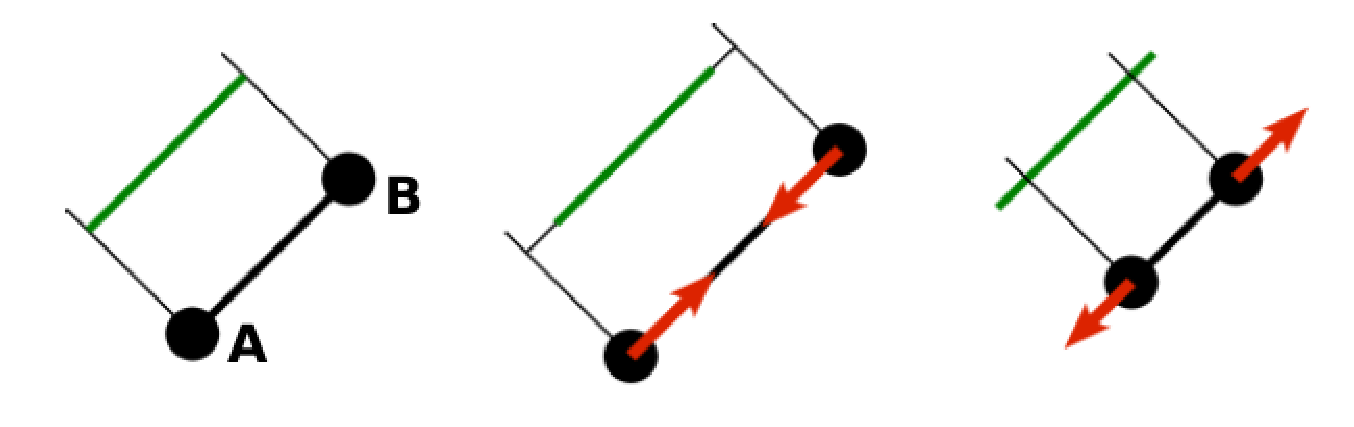
\includegraphics[width=0.7\textwidth]{figures/stretching.eps}
      \caption{Stretching force between two points of the mesh surface.}
\end{figure}
The stretching force acts between two particles and is symmetric. Therefore if an interaction is defined by
\begin{verbatim} 
inter 1 stretching_force 2.0 4.0
\end{verbatim}
then the following two commands
\begin{verbatim} 
part 42 bond 1 43
part 43 bond 1 42
\end{verbatim}
are equivalent.

\subsubsection{Bending force}
\textit{Syntax}\\
\hspace*{0.3 cm} $\mid$ \texttt{inter} $bondid$ \texttt{bending\_force} $\theta^0$ $k_b$ \\
\newline
\textit{Description}\newline

The tendency of an elastic object to maintain the resting shape is governed by prescribing the prefered angles between the neighbouring triangles of the mesh. This type of interaction is available for closed 3D immersed objects as well as for 2D sheet flowing in the 3D flow.


Denote by $\theta^0$ the angle between two triangles in the resting shape. For closed immersed objects, you always have to set the inner angle. The deviation of this angle $\Delta \theta = \theta - \theta^0$ is computed and defines two bending forces for two triangles $A_1BC$ and $A_2BC$
$$
F_{bi}(A_iBC) = k_b\frac{\Delta \theta}{\theta^0}n_{A_iBC}.
$$
Here, $n_{A_iBC}$ is the unit normal vector to the triangle $A_iBC$. The force $F_{bi}(A_iBC)$ is assigned to the vertex not belonging to the common edge. The opposite force divided by two is assigned to the two vertices lying on the common edge. This procedure is done twice, for $i=1$ and for $i=2$.

\begin{figure}[h]
   \centering
      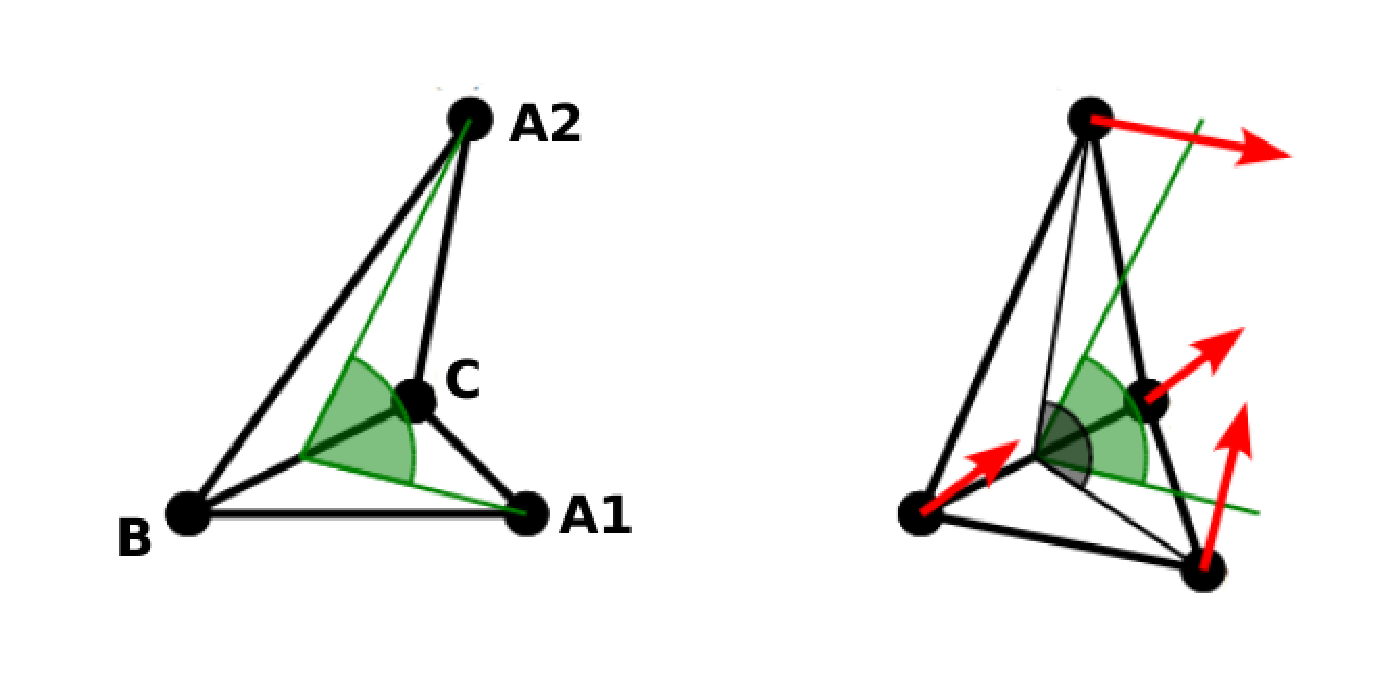
\includegraphics[width=0.7\textwidth]{figures/bending.eps}
      \caption{Bending force between two surface triangles.}\label{fig:bending}
\end{figure}

Unlike the stretching force the bending force is strictly asymmetric. After creating an interaction
\begin{verbatim} 
inter 33 bending_force 0.7 4.0
\end{verbatim}
it is important how the bond is created. Particles need to be mentioned in the correct order. Command
\begin{verbatim} 
part 0 bond 33 1 2 3
\end{verbatim}
creates a bond related to the angle between the triangles 012 and 123. In Figure \ref{fig:bending}, the particle 0 corresponds to point A1, particle 1 to C, particle 2 to B and particle 3 to A2. There are two rules that need to be fulfilled:
\begin{itemize}
\item there has to be an edge between particles 1 and 2
\item orientation of the triangle 012 must be correct, that is the normal vector defined as a vector product $01 \times 02$ must point to the inside of the immersed object.
\end{itemize}
Notice that also concave object can be defined. If $\theta_0$ is larger than $\pi$, then the inner angle is concave.

\subsubsection{Local area conservation}
\textit{Syntax}\\
\hspace*{3mm} $\mid$ \texttt{inter} $bondid$ \texttt{area\_force\_local} $S_{ABC}^0$ $k_{al}$ \\
\newline
\textit{Description}\newline

This interaction conserves the area of the triangles in the triangulation. This type of interaction is available for closed 3D immersed objects as well as for 2D sheet flowing in the 3D flow.

The deviation of the triangle surface $S_{ABC}$ is computed from the triangle surface in the resting shape $\Delta S_{ABC} = S_{ABC} - S_{ABC}^0$. The area constraint assigns the following  shrinking/expanding force to every vertex 
$$
F_{al}(A) = -k_{al}\frac{\Delta S_{ABC}}{S_{ABC}}w_{A}
$$
where $k_{al}$  is the area constraint coefficient, and $w_{A}$ is the unit vector pointing from the centroid of triangle $ABC$ to the vertex $A$. Similarly the analogical forces are assigned to $B$ and $C$. This interaction is symmetric, therefore after defining the interaction
\begin{verbatim} 
inter 44 area_force_local 0.02 4.0
\end{verbatim}
the following commands are equivalent
\begin{verbatim} 
part 0 bond 44 1 2
part 0 bond 44 2 1
part 1 bond 44 0 2
\end{verbatim}

\subsubsection{Global area conservation}
\textit{Syntax}\\
\hspace*{0.3 cm} $\mid$ \texttt{inter} $bondid$ \texttt{area\_force\_global} $S^0$ $k_{ag}$ \\
\newline
\textit{Description}\newline
This type of interaction is available solely for closed 3D immersed objects.

The conservation of local area is sometimes too restrictive. We add the global area constraint. Denote by $S$ the current surface of the immersed object, by $S_0$ the surface in the relaxed state and define $\Delta S = S - S_0$. Then we define the global area conservation force
$$
F_{ag}(A) = - k_{ag}\frac{\Delta S}{S}w_{A}
$$
Here, the above mentioned force divided by 3 is added to all three particles.

\begin{figure}[h]
   \centering
      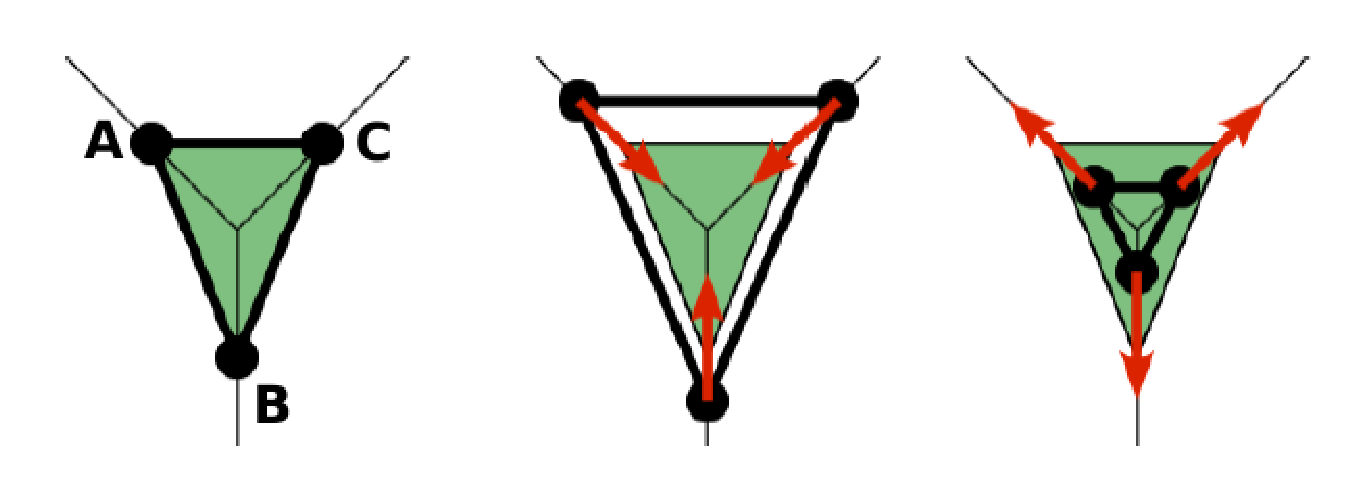
\includegraphics[width=0.7\textwidth]{figures/arealocal.eps}
      \caption{Local area force acting on a triangle of the mesh.}
\end{figure}
Again, this interaction is symmetric, as is the area\_{}force\_{}local.

\subsubsection{Volume conservation}
\textit{Syntax}\newline
\hspace*{0.3 cm} $\mid$ \texttt{inter} $bondid$ \texttt{volume\_forcel} $V^0$ $k_v$
\newline
\textit{Description}\newline
This type of interaction is available solely for closed 3D immersed objects.

The deviation of the global volume of the cell $V$ is computed from the volume in the resting shape $\Delta V = V - V^0$. For each triangle the following force is computed
$$
F_v(ABC) = -k_v\frac{\Delta V}{V^0} S_{ABC}\ n_{ABC}
$$
where $S_{ABC}$ is the area of triangle $ABC$, $n_{ABC}$ is the normal unit vector of plane $ABC$, and $k_v$ is the volume constraint coefficient. The volume of one immersed object is computed from
$$
V = \sum_{ABC}S_{ABC}\ n_{ABC}\cdot h_{ABC}
$$
where the sum is computed over all triangles of the mesh and $h_{ABC}$ is the normal vector from the centroid of triangle $ABC$ to any plane which does not cross the cell. The force $F_v(ABC)$ is equally distributed to all three vertices $A,B,C.$

\begin{figure}[h]
   \centering
      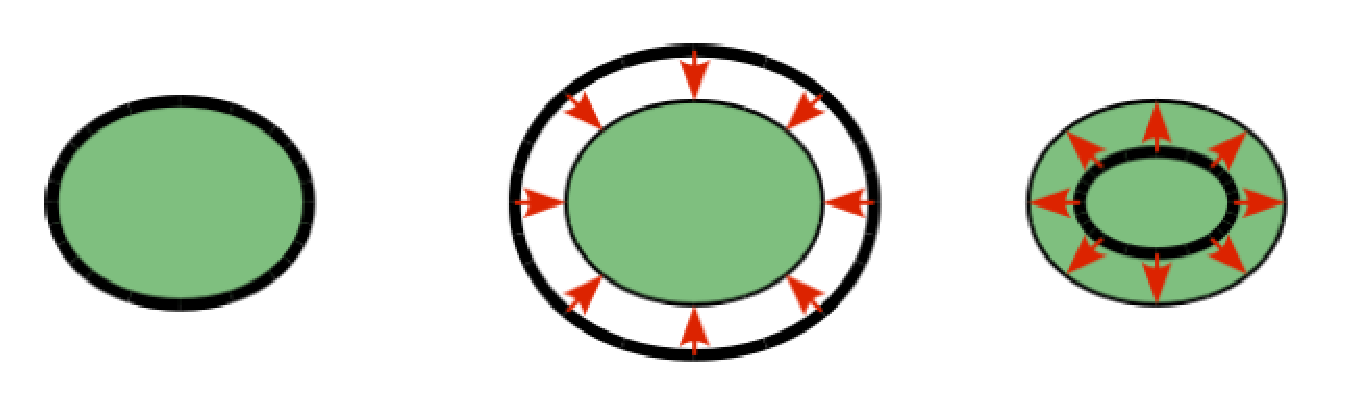
\includegraphics[width=0.7\textwidth]{figures/volume.eps}
      \caption{Volume force acting on the whole object.}
\end{figure}
This interaction is again non-symetric. After the definition of the interaction by 
\begin{verbatim} 
inter 22 volume_force 65.3 3.0
\end{verbatim}
we need to take care about the order of vertices. By the following command we define the bond
\begin{verbatim} 
part 0 bond 22 1 2
\end{verbatim}
Triangle 012 must have correct orientation, that is the normal vector defined by a vector product $01\times02$ must point inside the immersed object.

\section{Tcl example}
To demonstrate the usage of our implementation we show a tcl script. The script is to large extent self-explanatory. As the immersed object we use tetrahedron and red blood cell. In the \verb input \ directory, both triangulations are present.

In the beginning we set basic compulsory  ESPResSo parameters, such as \verb time_step ,\ \verb skin ,\ \verb box_l . Next we define the input directory together with the names of mesh files. 

Command \verb init_objects_in_fluid \ initialize the inner framework for working with immersed objects. 
Next comes the command \verb add_oif_object \ that actually creates the object. It takes several parameters. The compulsory parameters are 
origin, nodesfile, trianglesfile, type and mol. Optional arguments are mass, ks, kb, kal, kag, kv, rotate and stretch. 

Then we add the fluid to the system by \verb lbfluid \ command, prepare the vmd connection and then we run the simulation. 

In the main iteration loop we set the velocity of the fluid on the left side to a constant value. We run the \verb integrate \ command and repeat the main loop.

\begin{verbatim}
# general parameters
######################################

# whether to view the simulation on VMD
set vmd "y"

# integrator settings for the simulation
setmd time_step 0.1    
setmd skin 0.2
thermostat off

# rectangular channel box geometry
setmd box_l 100 20 20


# what files to read/generate where
######################################

# input files, describe the object shape
set inputdir "input"
# change these to one of the example files
# currently there are CELL and TETRA
set type [lindex $argv 0]
if {$type == ""} {
    set type "TETRA"
}
set fileNodes  "$inputdir/${type}mesh-nodes.dat"
set fileTriangles "$inputdir/${type}mesh-triangles.dat"

# initialization of the object-in-fluid mechanisms
######################################
init_objects_in_fluid	


# adding one object in fluid - oif. Some parameters are self-explanatory, some not:
######################################
add_oif_object origin 10 10 10 nodesfile $fileNodes trianglesfile $fileTriangles 
     stretch 1.0 1.0 1.0 ks 0.05 kb 0.01 kal 0.01 kag 0.01 kv 10.0 
     type 0 mol 0 rotate 0.0 0.0 0.0 mass 1.3
     


# origin            sets the coordinates of the center of the object
# stretch           the immersed object will be scaled 
#                   by these factors in the corresponding directions
# nodesfile         meshfile for vertices
# trianglesfile     meshfile for triangles
#
# elastic parameters of the object:
# ks    stretching of the cell
# kb    bending
# kal   local area preservation
# kag   global area preservation
# kv    volume preservation
#
# rotate    Rotation by specified angles around 
#           X axis, Y axis and Z axis. Angles given
#           in radians. rotateX=Pi/2 rotates the object 
#           by 90 degrees with the axes of rotation x 
#           such that vector 0,1,0 changes to 0,0,1 and
#           0,0,1 changes to 0,-1,0

# type      each immersed object must have 	
# mol       different type and mol ID


# run it!
######################################

lbfluid grid 1 dens 1.0 visc 1.5 tau 0.1 friction 0.5

if { $vmd == "y" } {
    prepare_vmd_connection simEspresso 3000 1
    exec sleep 2   
    imd positions
}

# main iteration loop

set cycle 0 
while { $cycle<200 } {
    puts "$cycle"
    if { $vmd == "y"} { imd positions }

    # setting the constant velocity
    # of the fluid on the left side of the md_box
    for { set i 0 } { $i < 1} { incr i } {
        for { set j 0 } { $j < 20 } { incr j } {
            for { set k 0 } { $k < 20 } { incr k } {
                lbnode $i $j $k set u 0.5 0.0 0.0
            }
        }
    }
    integrate 1
    incr cycle
}

\end{verbatim}

\section{Unresolved issues}\label{sec:unresolved}
\subsection{Variable viscosity}\label{subsec:viscosity}
%\item Question for Markus. For resolution btw immersed objects we use the notion mol\_id. However, now we expect, that all objects with a mol\_id are elastic objects. Our iterations run over all particles regardless if they belong to some immersed objects or not..... Is it a problem?
It would be great to implement the possibility to chose different density and viscosity of the fluid. We did some research in this direction, we also impemented an algorithm that can detect for every lbnode wheter it is located inside an immersed object or not. The implementation however was done for serial computation only, I suppose. It was also not tested yet.

\subsection{Different fluid-structure coupling}\label{subsec:coupling}
It is reasonable to try different approach in fluid-structure coupling. The currently implemented approach using the drag force between the fluid and spherical particles is in fact unphysical if one consideres movement of larger immersed object with particles being only a virtual sites on the membrane of that object. In this case, the immersed object moves only if there is a locally nonzero difference between the fluid velocity and the particle velocity. In other words, if there is a nonzero flow of the fluid through the membrane.

Other approach is in using the no-slip condition. Normally, fluid has zero velocity relative to the boundary. In other words, the local velocity of the fluid near the interface between fluid and structure is the same as the velocity of the particles. The interaction between the fluid and the immersed objects is not done  by transfer of the forces but by transfer of the velocities. 

It would be good to implement this in espresso and to compare both approaches.

\subsection{Orientation of the triangles}\label{subsec:orientation} 
It is possible to include a simple check whether all the triangles in the triangulation have correct orientation. This check can be included in the \verb add_oif_object \ procedure.

In some case, also if the triangle files are not given such that every triangle has good orientation, it is possible to restore good orientation. If we know the point in space inside the immersed object, from which we can see all the boundary points, then we can automatically verify the orientation of the triangles. It is thus possible to implement a simple check for this.

%\subsection{Restricted boundaries}\label{subsec:boundaries}
%We added functionality to creation of the boundaries. We added a range of validity for each component. For example, we want to make a \verb wall \ boundary at distance 3 with normal 1,0,0, but we want this boundary to be valid only for particles with z component in the range 5 to 10. The \verb constraint \ command allows us to create a plane
%\begin{verbatim}
%lbboundary wall dist 3 normal 1. 0. 0. type 0 
%\end{verbatim}
%This plane is however valid also for particles with z component of any value. We added switch \verb range , defining the range of validity of the constraint. It takes 6 arguments, namely xmin, xmax, ymin, ymax, zmin, zmax, with first two arguments defining minimal and maximal x-coordinate, for which the constraint is valid. Remaining 4 parameters have analogous meaning. To create a boundary waal which is valid for particles only with z coordinate in range 5 to 10, we write
%\begin{verbatim}
%lbboundary wall dist 3.5 normal 1. 0. 0. type 0 
           %range -10000 10000 5 10 -10000 10000
%\end{verbatim}
%This way it is possible to create concave boundaries, for example:
%\begin{verbatim}
%setmd box_l 10 10 10
%constraint wall dist 0 normal -1 0 1 type 0 range 0 5 -1000 1000 -1000 1000
%constraint wall dist 10 normal 1 0 1 type 0 range 5 10 -1000 1000 -1000 1000
%\end{verbatim}
%Here, a concave channel is created. Its shape in the xz direction is depicted in Figure \ref{fig:concave}.
%\begin{figure}[h]
   %\centering
      %\includegraphics[width=0.4\textwidth]{figures/boundary.eps}
      %\caption{Concave channel, its projection onto xz plane.}\label{fig:concave}
%\end{figure}


\begin{thebibliography}{1}

\bibitem{Cimrak2011a}
I.~Cimr\'ak, M.~Gusenbauer, and T.~Schrefl.
\newblock Modelling and simulation of processes in microfluidic devices for
  biomedical applications.
\newblock {\em Computers an Mathematics with Applications}.
\newblock Doi:10.1016/j.camwa.2012.01.062.

\bibitem{Dao2003}
M.~Dao, C.T. Lim, and S.~Suresh.
\newblock Mechanics of the human red blood cell deformed by optical tweezers.
\newblock {\em J. Mech. Phys. Solids}, 51:2259--2280, 2003.

\bibitem{Dupin2007}
M.M. Dupin, I.~Halliday, C.M. Care, and L.~Alboul.
\newblock Modeling the flow of dense suspensions of deformable particles in
  three dimensions.
\newblock {\em Phys Rev E Stat Nonlin Soft Matter Phys.}, 75:066707, 2007.

\end{thebibliography}

\end{document}
